\begin{center}
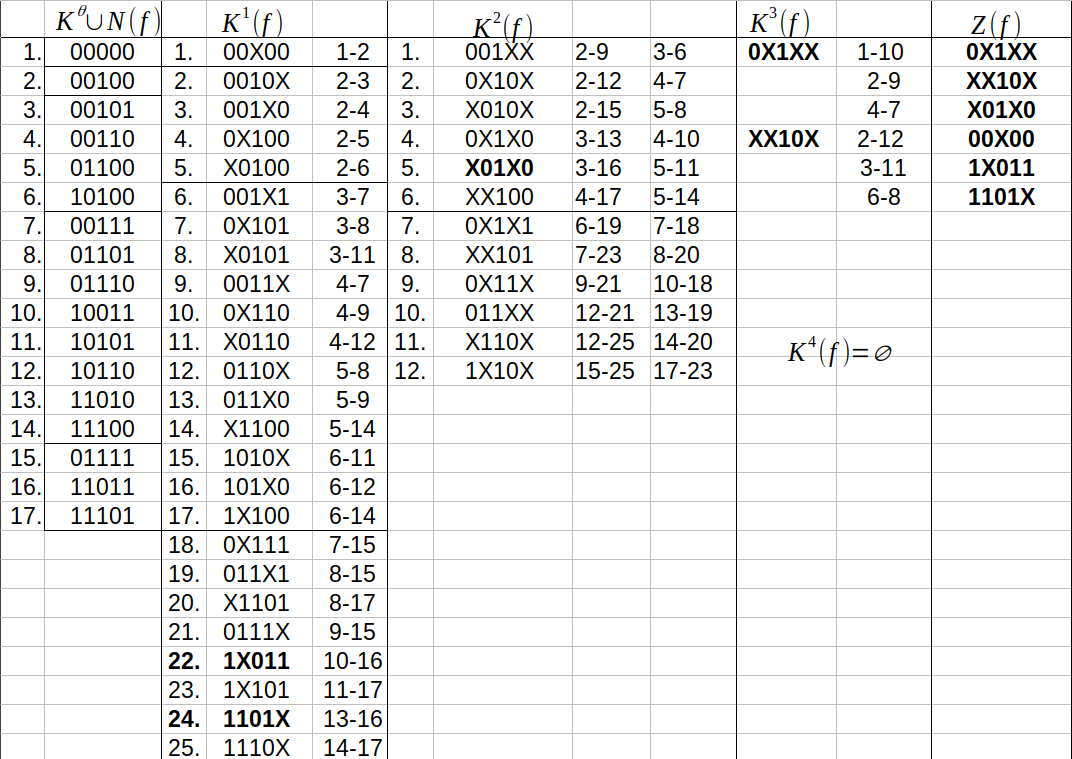
\includegraphics[width=\linewidth]{imgs/kvain_mak_table.png}
\end{center}
\par\textit{Составление импликантной таблицы}

Импликантная таблица в первоначальном виде содержит 6 строк (по числу 
простых импликант) и 13 столбцов (по числу существенных вершин).

\begin{center}
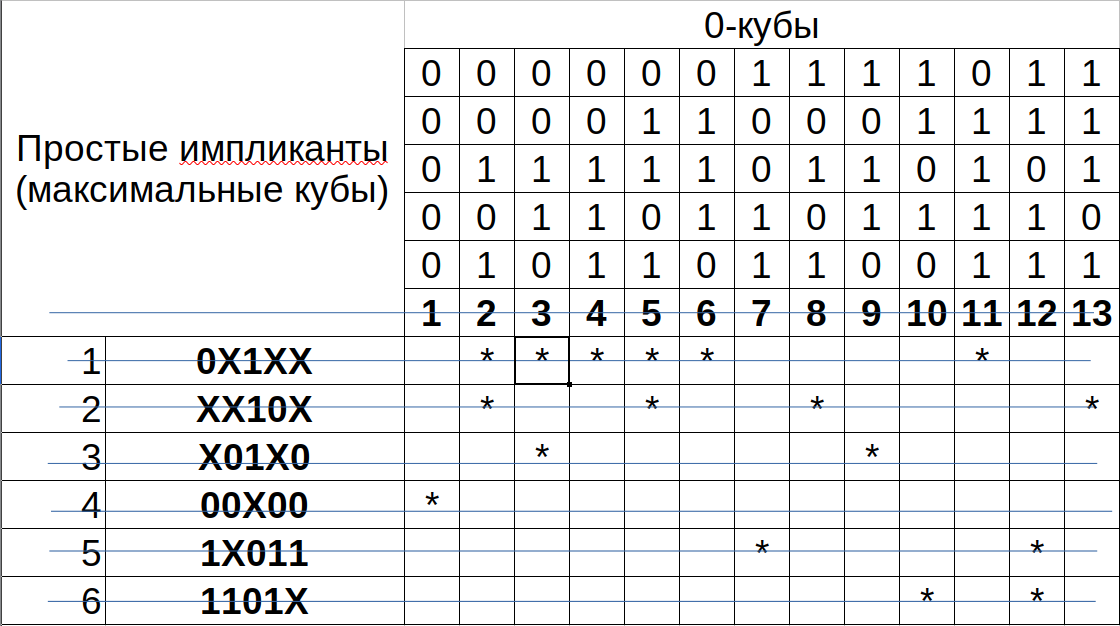
\includegraphics[width=0.6\linewidth]{imgs/implicant_table.png}
\end{center}

Все существенные вершины покрываются покрываются существенными импликантами.
\begin{equation*}
  C_{min}(f)= 
  \begin{Bmatrix}
    0 & X & 1 & X & X \\
    X & X & 1 & 0 & X \\
    X & 0 & 1 & X & 0 \\ 
    0 & 0 & X & 0 & 0 \\ 
    1 & X & 0 & 1 & 1 \\ 
    1 & 1 & 0 & 1 & X 
  \end{Bmatrix}
  \begin{pmatrix}
    1 \\ 2 \\ 3 \\ 4 \\ 5 \\ 6
  \end{pmatrix}
  S^a = 19; \hfill S^b = 25
\end{equation*}

МДНФ имеет следующий вид: \\
$ f = \
\nx{1}\x{3} \vee \
\x{3}\nx{4} \vee \
\nx{2}\x{3}\nx{5} \vee \
\nx{1}\nx{2}\nx{4}\nx{5} \vee \
\x{1}\nx{3}\x{4}\x{5}  \vee \
\x{1}\x{2}\nx{3}\x{4} \
$